%
% Chapter 7
%

\chapter{BACKGROUND PREDICTIONS}
\label{chap:background}
Despite optimizing the event selection criteria to select signal events, a substantial amount of background from a variety of processes enters the signal region.
These backrounds are classified as being either reducible or irreducible, and are estimated differently depending on this classification. An understanding
of each background process and a proper assessment of the uncertainity associated with the estimation of each background is critical to extracting the signal and interpreting
the results. 

\section{Reducible Backgrounds}
Reducible backgrounds arise from a number of sources, but always contain leptons that are either non-prompt, or have a lepton whose electric charge is mismeasured.
These backgrounds are classified as reducible because if the event selection and CMS object reconstruction worked with perfect efficiency, the events would not
enter the signal region; thus, improving the prompt lepton identifiction and CMS lepton electric charge measurement can reduce the contributions from these processes.
Reducible backgrounds are estimated via data-driven approaches using control regions and extrapolation techniques to predict their contribution to the yield in the
signal region. The background due to fakes is entirely separate from the charge mismeasurement background and are estimated separately. 

\subsection{Fake Lepton Background} 
The fake lepton background gets its name from the fact that events with non-prompt leptons pass the tight selection and enter the signal region by faking prompt leptons. These
fakes typically originate from leptonic decays of certain hadrons, such as the B, D, $\Lambda$, and K. The primary source is the relatively large cross-section semi-leptonic \ttbar
process, where the b-jet from the leptonic top quark produces a fake lepton that passes the tight lepton selection criteria, but also includes other processes where a lepton
is produced inside a jet. The background from these events is estimated via a loose-to-tight extrapolation. This begins with measuring the rate at which the leptons passing
the fakeable selection also pass the tight selection, known as the fake rate. The measurement is performed in a control region of the data, known as the measurement region (see below).
The measurement is then used to extrapolate from a sideband with fakeable leptons to estimate the contribution in the signal region 
from events with fake leptons. 

The measurement region is heavily enriched in QCD multijet events, which provide a
source of mostly fake leptons. The fake rate is defined as the probability of a non-prompt lepton which passes the fakeable selection to also pass the tight selection.
The measurement region events satisfy the following requirements:

\begin{itemize}
 \item exactly one fakeable lepton
 \item one preselected jet with $\Deta$R $>$ 0.7 from the lepton
 \item $M_{T}(l,\met) < 15$ GeV
\end{itemize}

\noindent This selection enriches the measurement region with non-prompt leptons. The data analyzed in the measurement region is collected on single lepton
triggers which require a single lepton and a particle-flow jet with \pt $>$ 30 GeV.

To ensure a high purity of fake leptons in the measurement region, the contribution of prompt leptons must be accounted for. This contribution arises from W and Z plus jets processes, but also from \ttbar. The Z contamination
is addressed by vetoing events with more than one loose lepton. The prompt leptons from W decays is subtracted with a fit to the transverse mass of the lepton and missing energy, $M_{T}(l,E_{T}^{miss})$. A cut is first applied requiring
$M_{T}(l,E_{T}^{miss}) < $15 GeV, with the residual contamination subtracted in each \pt bin using W/Z +jet MC. 

The final fake rates are shown in Figure~\ref{fig:fakerate}. The larger uncertainties for higher \pt leptons is due to the larger uncertainties from the prompt lepton subtraction method. A good agreement between data and MC is observed overall.
In this analysis, electrons from photon conversions are treated as a separate background and estimated via MC. The fake rate in the measurement region for electrons is scaled by the ratio of fake rate including electrons from conversions to
the fake rate excluding electrons from conversions from QCD MC. 

\begin{figure}[htp]
\centering
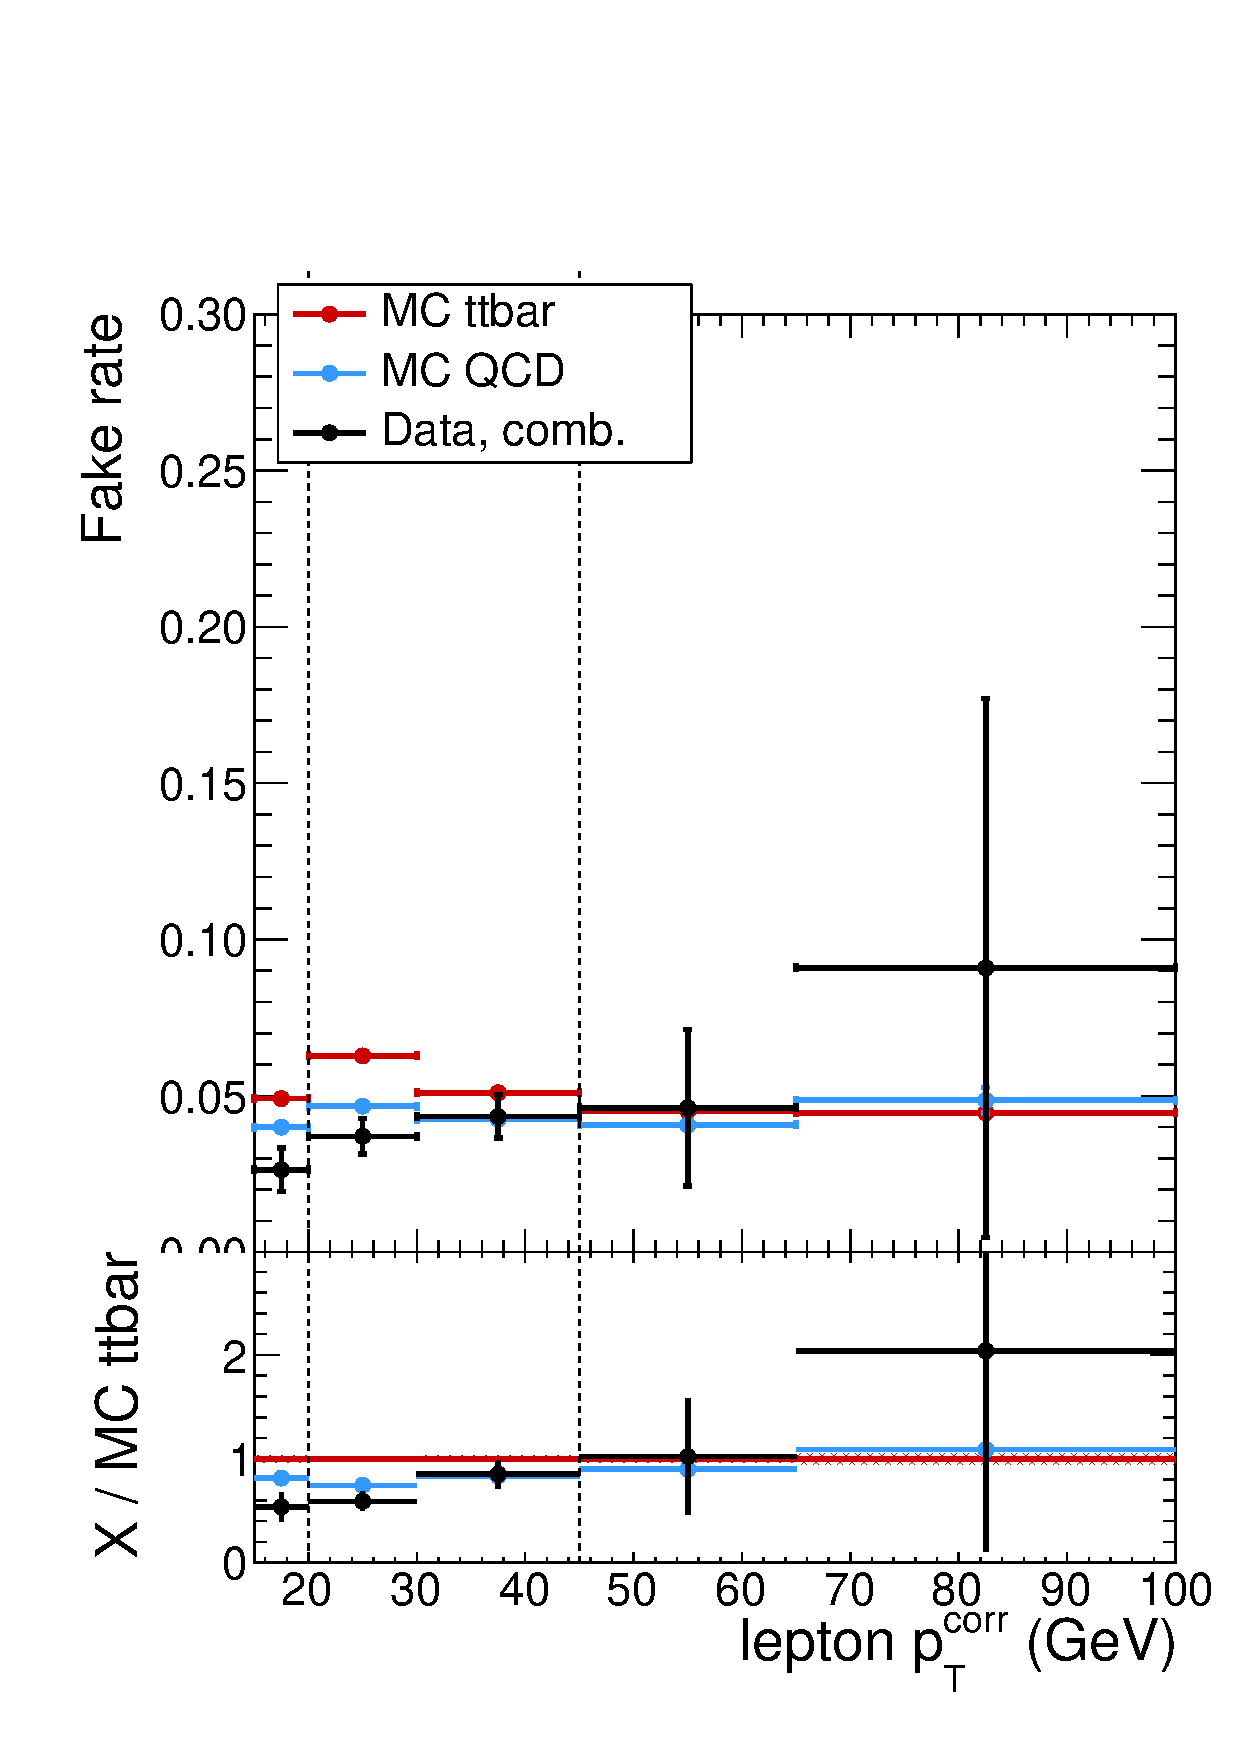
\includegraphics[width=0.39\textwidth]{ch7_figs/fr_mu_barrel.pdf}
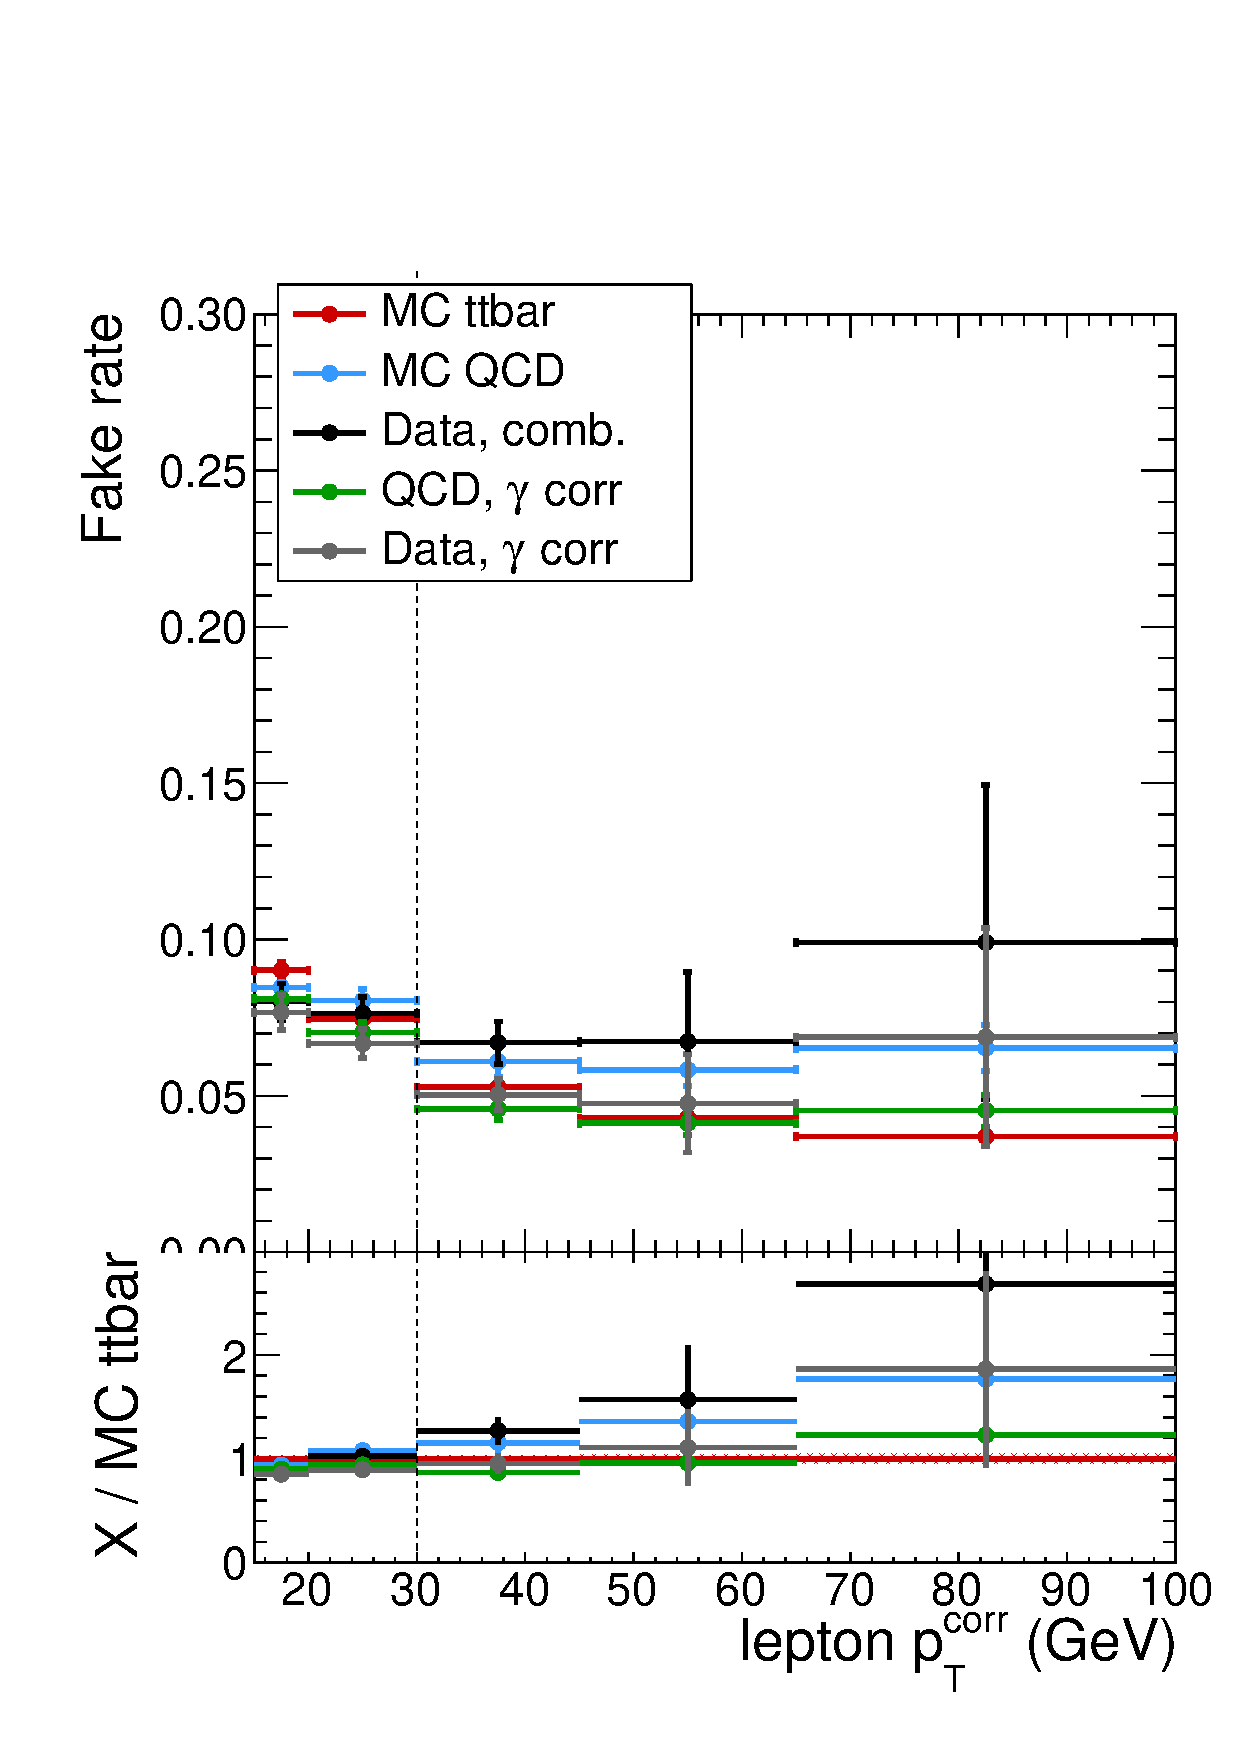
\includegraphics[width=0.39\textwidth]{ch7_figs/fr_el_barrel.pdf}\\
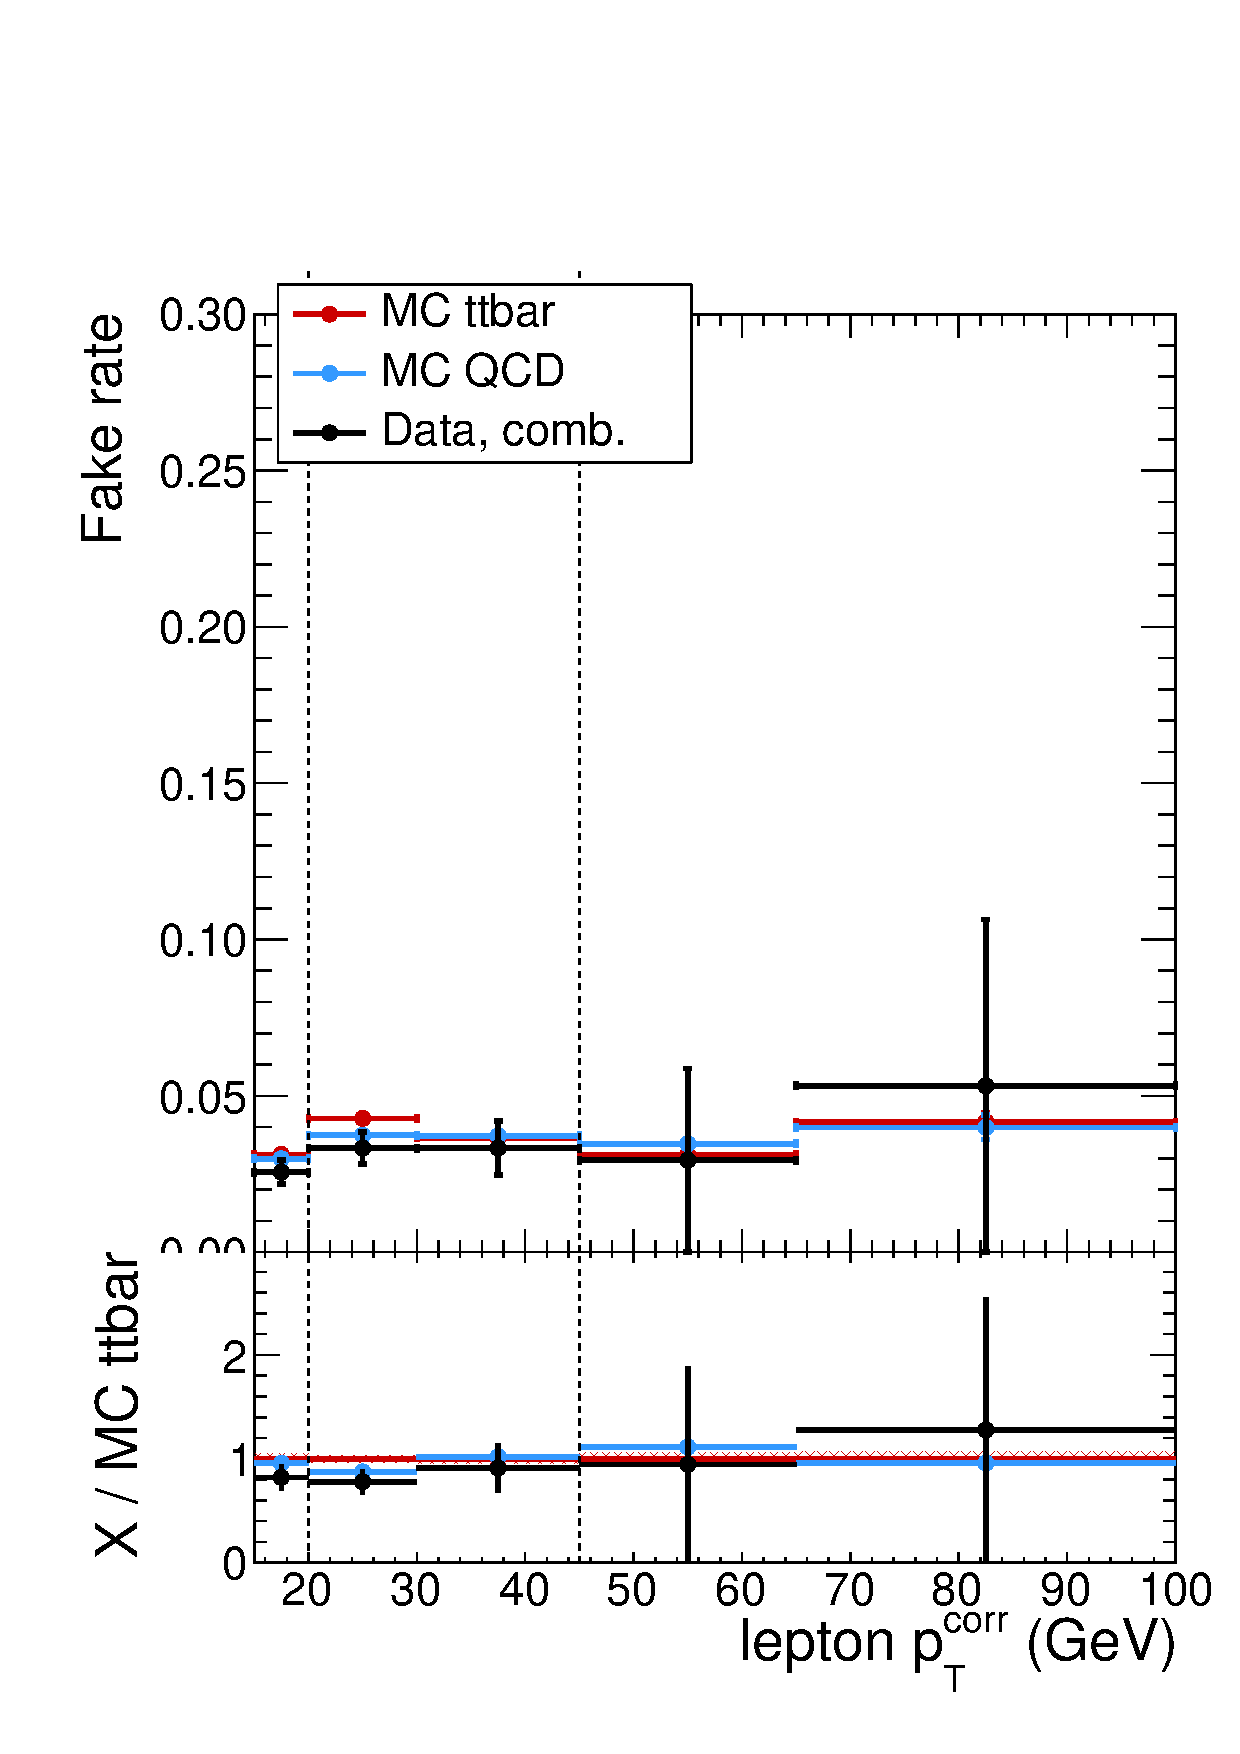
\includegraphics[width=0.39\textwidth]{ch7_figs/fr_mu_endcap.pdf}
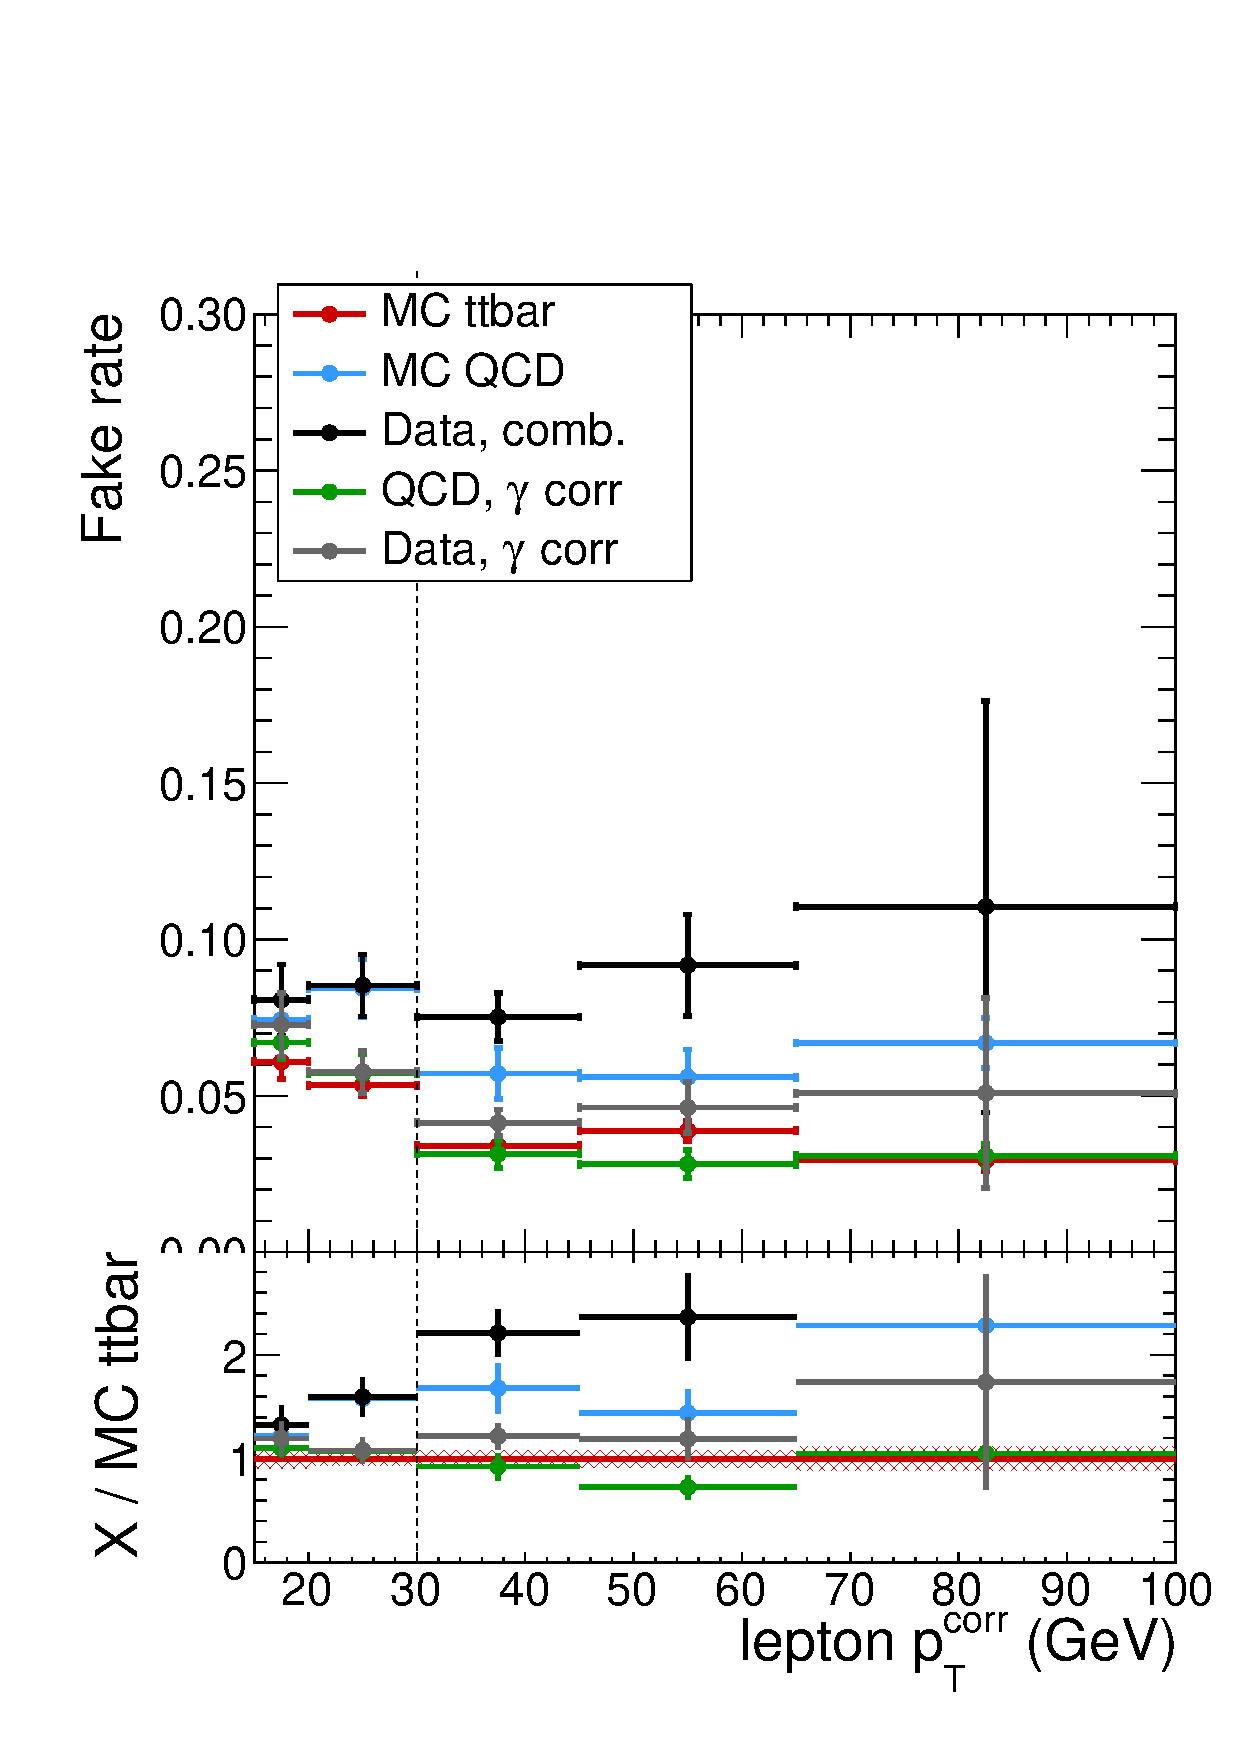
\includegraphics[width=0.39\textwidth]{ch7_figs/fr_el_endcap.pdf}
\caption[Fake rate measurements in data and MC.]{The lepton fake rates as measured in data and QCD as well as \ttbar MC. Fake rates for muons are on the left while fake rates for electrons are on the right. The fake rates
measured in the barrel are on the top while the fake rates measured in the endcaps are on the bottom.}
\label{fig:fakerate}
\end{figure}

Once the fake rate is obtained from the measurement region, it is applied in a second control region, also enriched in fakes, denoted as the application region. The weighted yields in this region constitute the background due to
fake leptons in the signal region. As such, the application region is identical to the signal region, except that the requirement of the two same-sign leptons passing the tight selection is relaxed to passing the fakeable selection,
and that at least one of these leptons fails the tight selection. The fake rate weights are expressed
in terms of event yields as a function of the number of leptons failing the tight selection in a given event. The contribution of fakes in the signal region is estimated using equation~\ref{eqn:fake_rate} below:

\begin{equation}
\label{eqn:fake_rate}
  N_{pp}^{bkg} = \frac{f_{1}}{1-f_{1}}N_{pf} + \frac{f_{2}}{1-f_{2}}N_{pf} - \frac{f_{1}f_{2}}{(1-f_{1})(1-f_{2})}N_{ff}
\end{equation}

\noindent under the assumption that the contribution of prompt leptons failing the tight selection is negligible with respect to the number of non-prompt leptons failing. Here, $N_{pp}^{bkg}$ is the background contribution from fake leptons
in the signal region, $f_{1,2}$ is the fake rate for the leading, subleading lepton calculated from the measurement region, $N_{pf}$ is the number of events in the application region with 1 prompt and 1 fake lepton, and $N_{ff}$ is the
number of events in the application region with two fake leptons.

%%%%%%% explanation for cone pt %%%%%%%%%%%%%%%%
The fake lepton background estimation method described above is valid only for leptons which pass the trigger, because the fake rate was measured using leptons passing the trigger.
This is important because although the measurement region contains only leptons which pass the trigger, the application region consists of some events which contain one lepton passing the trigger and one that fails the trigger.
The method described above biases these events because the fake rate assigned to the lepton not passing the trigger is incorrect.
Because this background estimation method relies on the fake rates in the measurement region and the application region to be the same,
the fakeable object definition must not depend on whether or not the lepton passed the trigger.
To remove this bias, we use a quantity called the ``corrected'' \pt in place of the
standard \pt.  The corrected \pt is the same as the standard \pt if the lepton passes the tight selection, but modified to 0.9 times the nearest jet \pt otherwise. 
The trigger bias was explicitly checked in lepton-enriched QCD MC events, 
where the fake rate is studied with and without requiring the lepton to pass the trigger. This study showed that the trigger turn-on curve requires the trigger \pt threshold to be significantly lower than
the corrected \pt to avoid any bias.
Thus the fake rate is measured independently in bins of corrected lepton \pt for events collected by each trigger in the measurement region. The triggers used to avoid any bias in the corrected \pt are listed
with each \pt bin below in Table~\ref{tab:fakerate_triggers}.

\begin{table}[hbtp]
\centering
\caption{Corrected \pt range and corresponding trigger categories for each bin of the fake rate measurement.}
\begin{tabular}{l|l}
\hline
Corrected \pt [GeV] & Trigger \\
\hline
10$< \pt(\mu) < $20 & \textsc{HLT$\_$Mu3$\_$PFJet40} \\
20$< \pt(\mu) < $45 & \textsc{HLT$\_$Mu8} \\
$\pt(\mu) > $45 & \textsc{HLT$\_$Mu17} \\
\hline
15$< \pt(e) < $20 & \textsc{HLT$\_$Ele8$\_$CaloIdM$\_$TrackIdM$\_$PFJet30} \\
20$< \pt(e) < $30 & \textsc{HLT$\_$Ele12$\_$CaloIdM$\_$TrackIdM$\_$PFJet30} \\
$\pt(e) > $30 & \textsc{HLT$\_$Ele17$\_$CaloIdM$\_$TrackIdM$\_$PFJet30} \\
\end{tabular}
\label{tab:fakerate_triggers}
\end{table}


\subsection{Charge Mismeasurement Background}
One of the defining requirements of the signal region is that the two leptons have the same-sign electric charge. This requirement makes leptons where the charge was mismeasured an important background. Like the background due to fake leptons,
this background is also estimated from data with two control regions: the first for measuring the rate of charge mismeasurments (also known as charge flips), and the second for applying the weights derived from the first to extrapolate to
the signal region. Unlike the fake background however, the charge mismeasurement background is only comprised of events with electrons, as the probability for mismeasuring the electric charge of a muon is negligible.

The control region used for measuring charge flip probabilities is defined by selecting Z$\rightarrow$ee events in data. Here it is assumed that same-sign electron pairs within 10 GeV of the Z peak are due to a charge mismeasurement of one of
the electrons. Charge flip probability measurements are performed by measuring same-sign yields to opposite sign yields in the Z peak and are parameterized as a function of electron \pt and $\eta$.
The yields are determined from a fit to the Z invariant mass shape, which is modeled with the convolution of a crystal ball and Breit-Wigner function for the signal and an exponentially falling function for the background. 
The measurement is performed in 3 bins of \pt (10-25 GeV, 25-50 GeV, and $\geq$50 GeV), and two bins of $\eta$ ($\leq$ 1.479, and $>$ 1.479) for a total of 21 categories of electron pairs. Each category corresponds to the \pt-$\eta$ bin
of the leading lepton, and the \pt-$\eta$ bin of the subleading electron.  
The charge flip probabilities are determined from a simultaneous fit to the 21 same-sign and opposite-sign yields. The resulting charge flip probabilities range between approximately 0.03$\%$ in the barrel
to approximately 0.4$\%$ in the endcaps and are summarized in Figure~\ref{fig:fliprate} below.

\begin{figure}[htp]
\centering
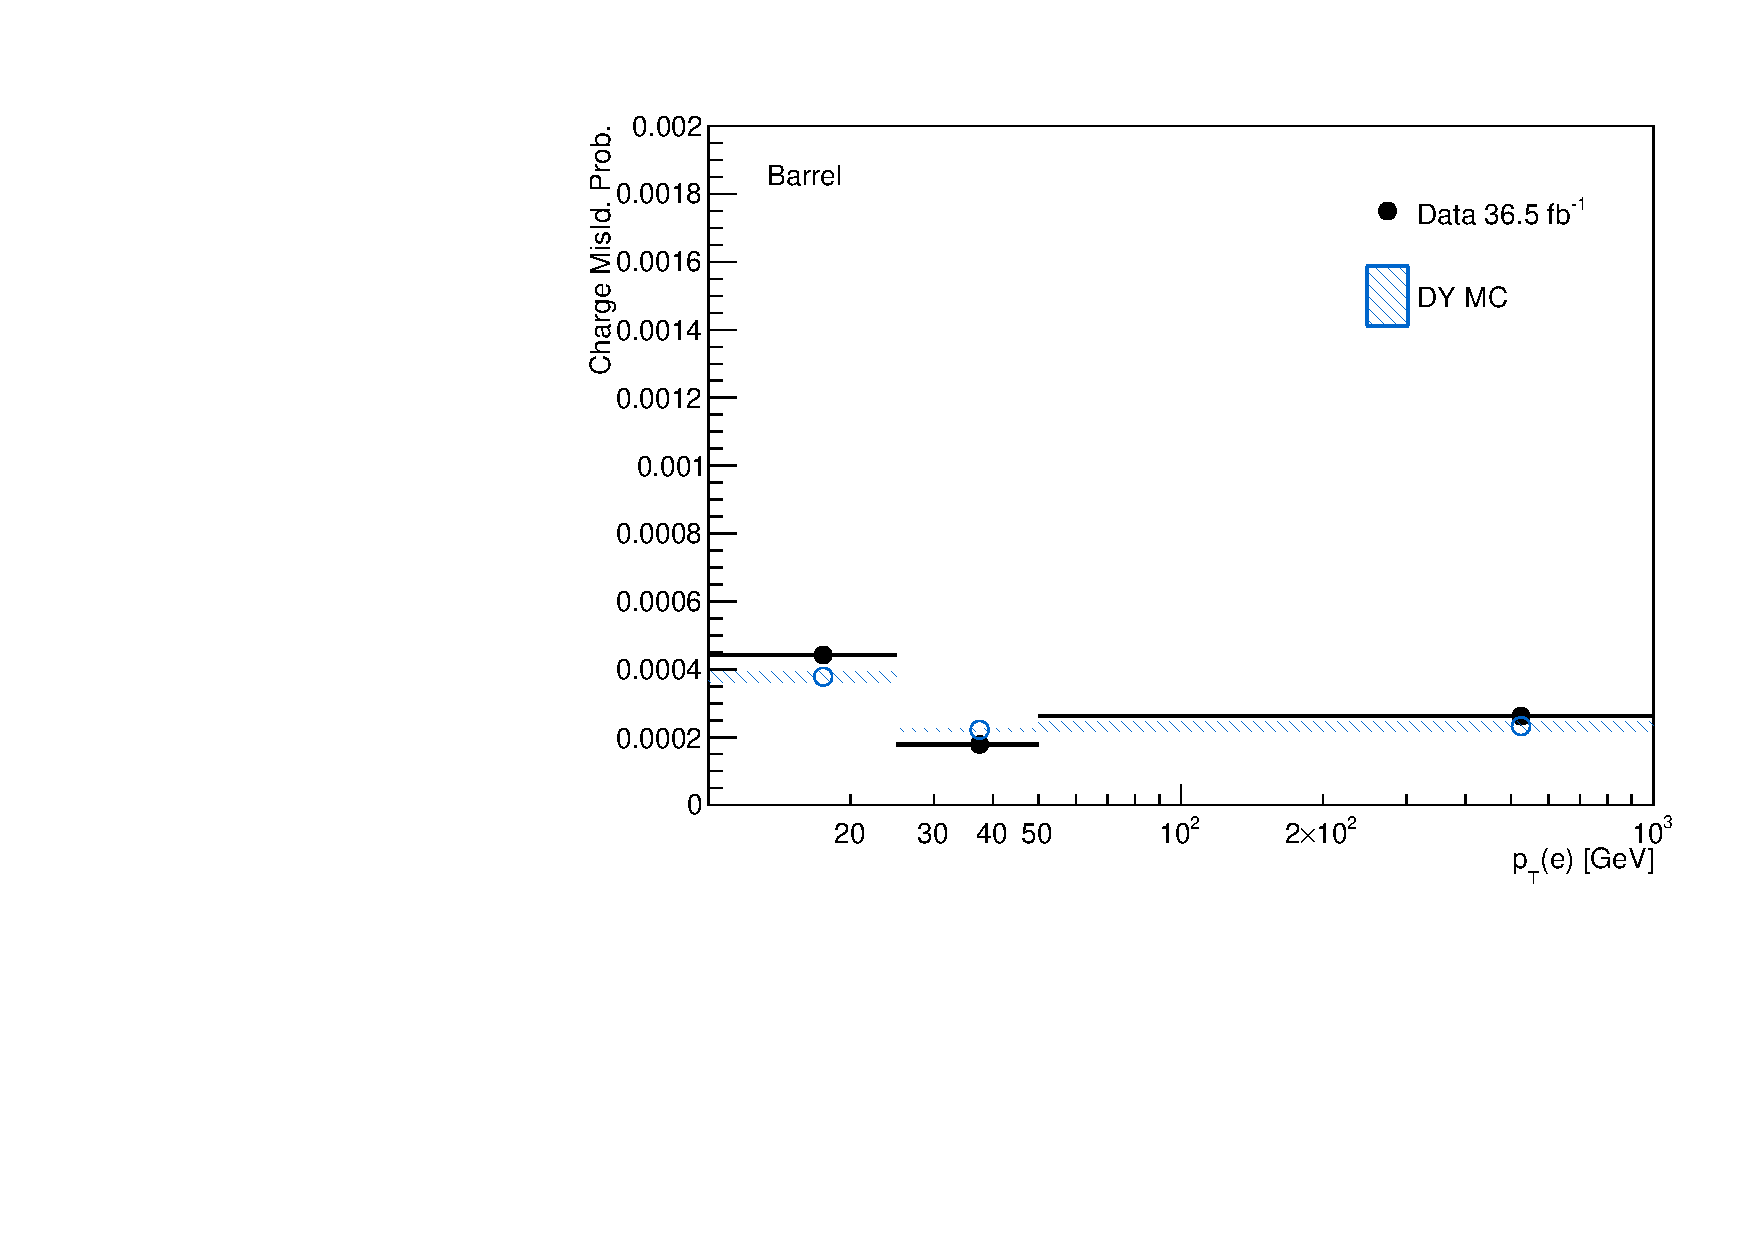
\includegraphics[width=0.49\textwidth]{ch7_figs/chmid_prob_barrel.pdf}
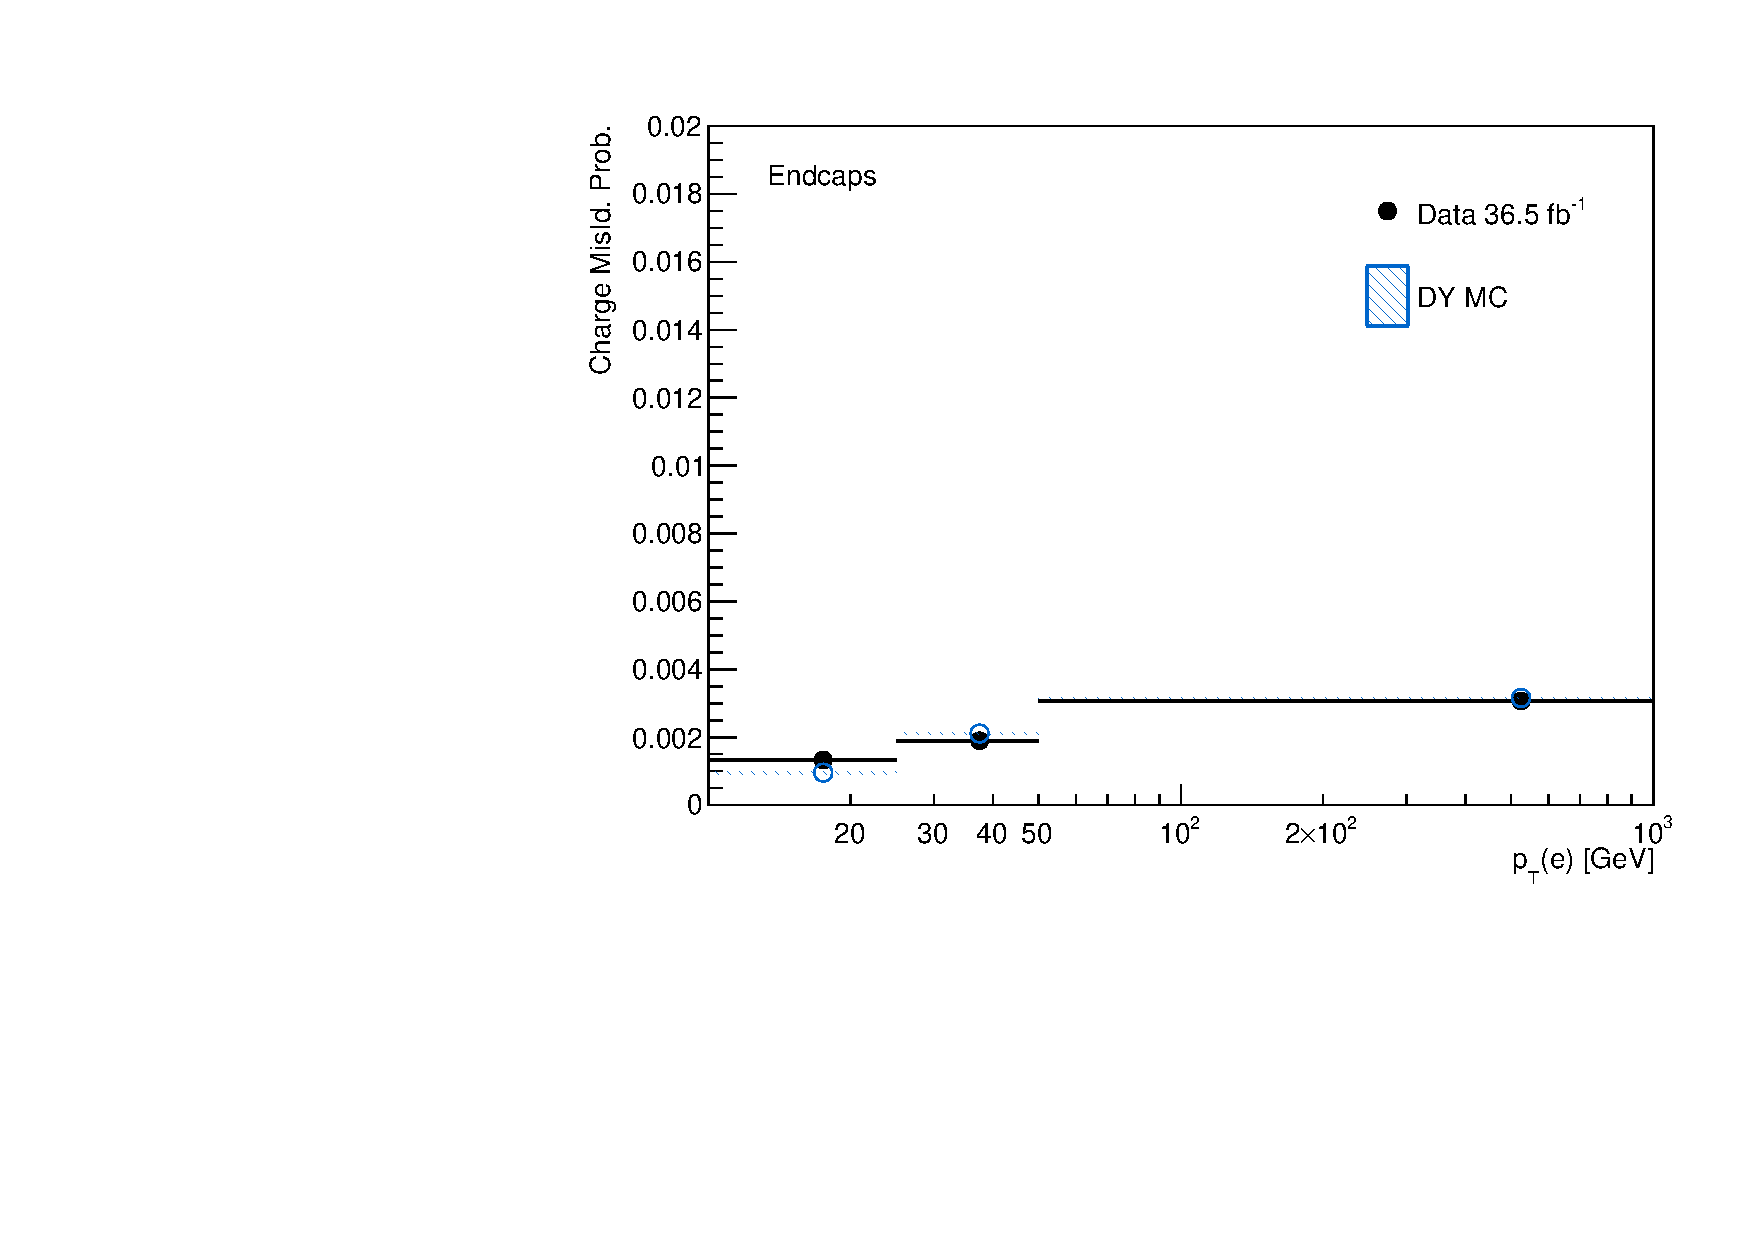
\includegraphics[width=0.49\textwidth]{ch7_figs/chmid_prob_endcap.pdf}\\
\caption[Electron charge misassignment probabilities in data and MC.]{Charge misassignment probabilities as a function of \pt for electrons in the barrel (left) and endcaps (right).}
\label{fig:fliprate}
\end{figure}
 
The control region where the charge flip probabilities measured above are applied must extrapolate well to the signal region to provide an accurate background estimation. As such, this control region
is identical to the signal region except that the same-sign charge requirement on the leptons is replaced with an opposite-sign requirement.
The charge misassignment probability $P(\pt,\eta)$ is applied per lepton. The total event weight is then $P_{1} + P_{2}$ in the $ee$ category, and $P$ in the $e\mu$ category.  

\section{Irreducible Backgrounds}
Irreducible backgrounds are estimated exclusively from MC. Irreducible backgrounds earn their name from the fact that even if the signal region selection and CMS event/object reconstruction
worked with perfect efficiency and purity, these backgrounds still produce the necessary objects to consistently pass the signal region selection and are thus irreducible with respect to the signal
region definition. The dominant irreducible background processes include \ttw and \ttz. Other irreducible background processes include diboson pairs produced in association with jets,
while smaller contributions include processes with a single W or Z boson, a single top quark, tribosons, as well as other rare\footnote{Rare means a very small cross section, and very
small yield in the signal region.} SM backgrounds. The modelling of these background processes has been checked to ensure a good agreement among the variables used to event selection and
signal extraction.  

While the signal region selection vetoes events with low mass dilepton pairs, the $t\bar{t}\gamma^{*}$ process with $\gamma^{*}\rightarrow l^{+}l^{-}$ still contributes as a background when one of the leptons fails
selection cuts or is out of the acceptance. The nominal \ttz sample is generated with $m_{l^{+}l^{-}} >$ 10 GeV, and we therefore use a $t\bar{t}Z/\gamma^{*}$ sample generated at 1 $< m_{l^{+}l^{-}} <$ 10 GeV
and an additional \ttbar sample which covers the $ m_{l^{+}l^{-}} <$ 1 GeV phase space. The \ttbar sample is generated with MadGraph and showered with Pythia, which can decay a low-virtuality $\gamma^{*}$.

Although electrons from conversions are technically a reducible background, they are estimated from MC. This is because the background from conversions, primarily $t\bar{t}\gamma$, can have events where one conversion
electron is not reconstructed, and the other is mistakenly identified as a prompt, isolated electron\footnote{When both conversion electrons are reconstructed, the conversion veto applied in the tight electron selection
rejects both.}. Because these leptons look more prompt-like compared to typical fakes, they are not estimated well with the fake-rate method. For the conversion backgrounds, MC is used and normalized to NLO QCD cross section
from \textsc{MadGraph5$\_$aMC$\@$NLO}.

%% \begin{figure}[hbtp]
%%  \begin{center}
%%    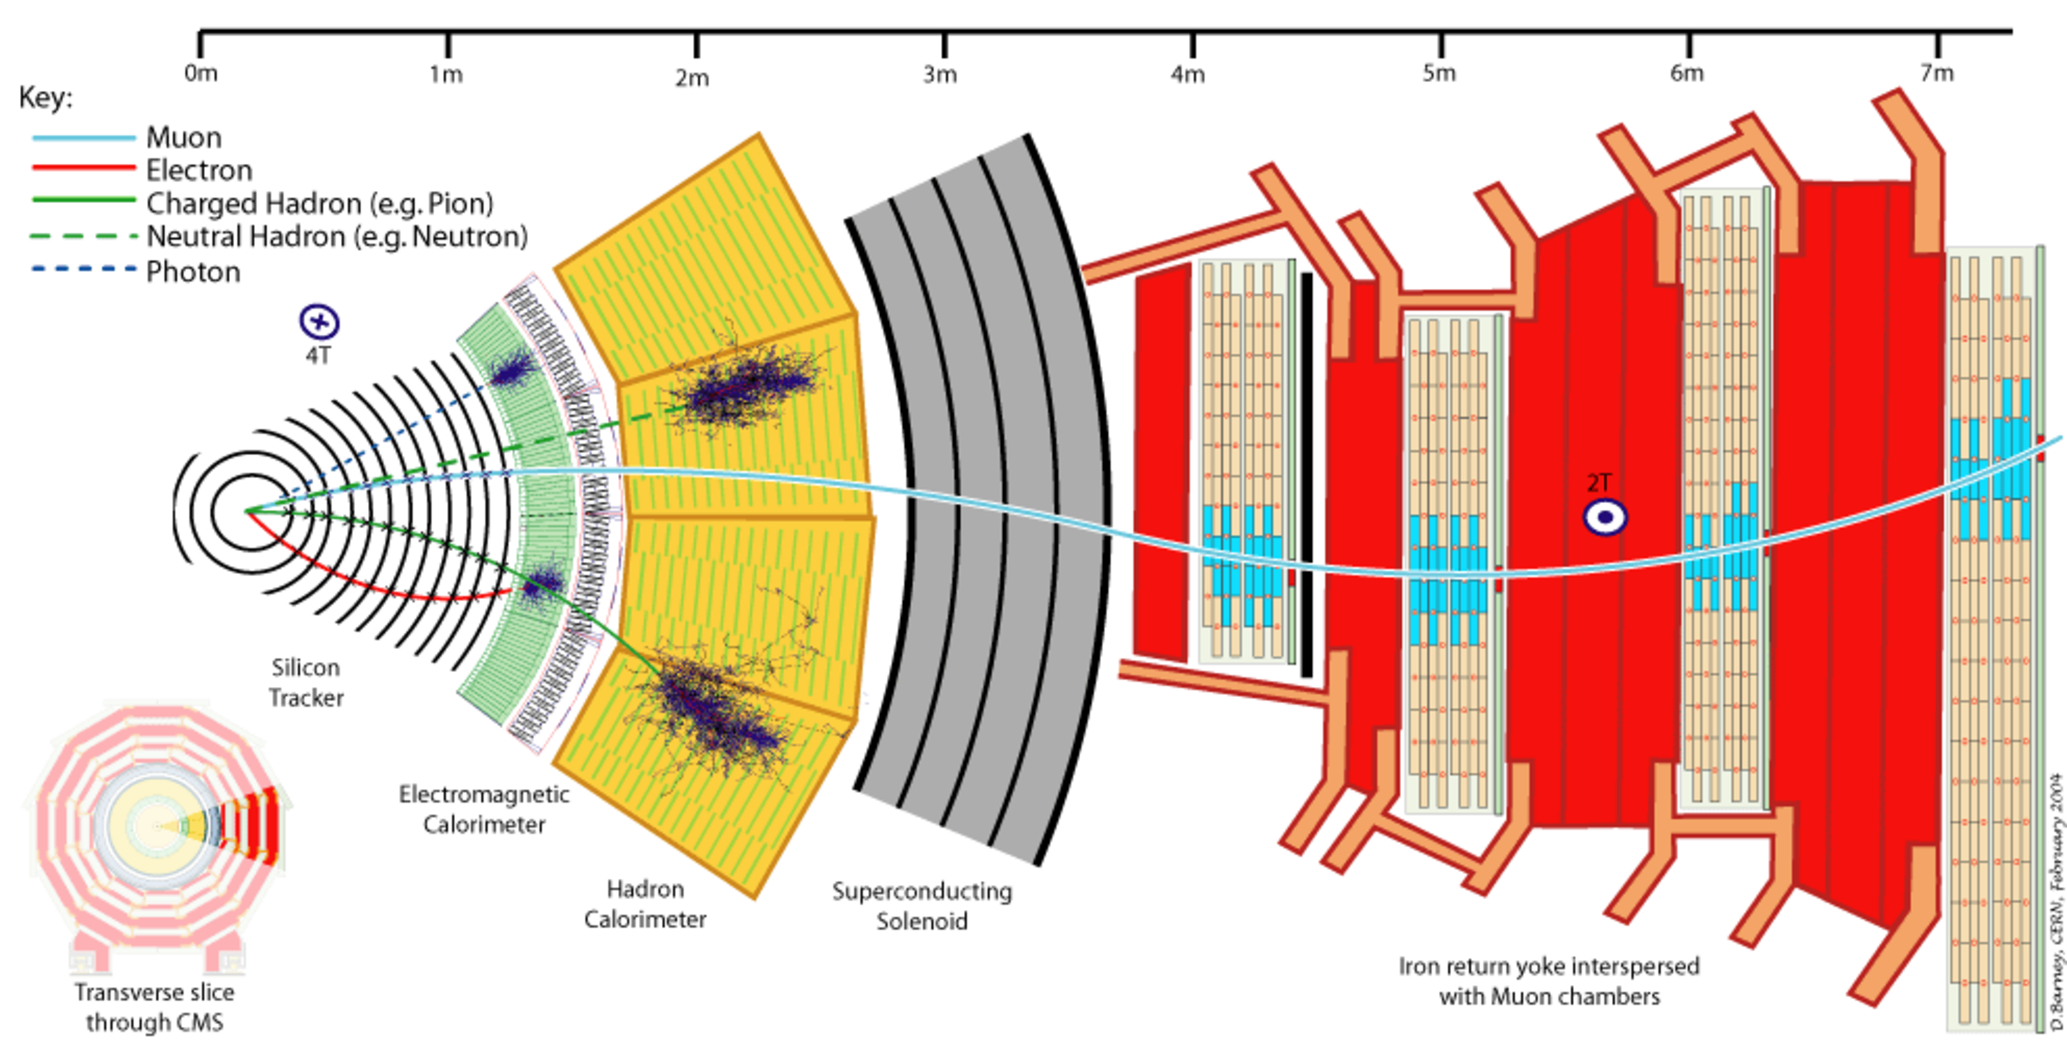
\includegraphics[width=0.8\textwidth]{ch4_figs/cms_particleflow.pdf}
%%    \caption{An overview of how CMS detects different types of particles. The slice of CMS in in the x-y plane.~\cite{NEED CITATION}.}
%%    \label{fig:cms_pflow}
%%  \end{center}
%% \end{figure}
